\documentclass[12pt]{article}
\usepackage[brazilian]{babel} %traduz para o pt-br
\usepackage[utf8]{inputenc} %reconhece acentua\c{c}\~{a}o
\usepackage{lipsum} %gera textos aleat\'{o}rios
\usepackage{graphicx} %uso de imagens
\usepackage{amssymb} % para exibir simbolos matematicos
\usepackage{subfig} %uso de caixa de figuras
\usepackage{amsmath} %para usar begin{cases}
\usepackage{amsfonts} %para usar mathbb
\usepackage{float} %fixa tabela e imagens flutuantes
\graphicspath{{images/}} %diretorio onde ficar\~{a}o imagens
\usepackage{latexsym}
\usepackage{lineno} %para mostrar numeração de linhas

%opening
\title{Análise Combinatória, Probabilidades e Aplicações - Lista 03}
\author{{Cleibson Aparecido de Almeida}}

\begin{document}

\maketitle

\section*{Exercício 01 - Para cada um dos experimentos abaixo, descreva o espaço amostral $\Omega$ adequado e apresente o número de elementos, quando for o caso.}


\subsection*{a - Um dado é lançado três vezes e a sequência de números obtida é anotada.}

$\Omega = \{A \subseteq \{1,2,3,4,5,6\}: |A|=3\}$

Considerando que são 6 possibilidades para cada lançamento do dado e faremos 3 lançamentos, então teremos $6^3=216$ elementos. Não será descrito todo o conjunto devido ao seu tamanho ser grande. Porém $\Omega = \{ \{1,1,1 \}, \{1,1,2 \}, \{1,1,3 \},..., \{6,6,6 \} \}$.

\subsection*{b - Numa determinada cidade, no mês de março, conta-se o número de problemas nas tubulações de água do bairro x.}

$\Omega = \{B \subseteq \{0,1,2,3,...,n\}: |B|=1\}$

Neste caso, teremos $n+1$ elementos. 

Obs: Se considerar um conjunto de infinitos elementos, pode-se considerar que $n \rightarrow \infty$ e neste caso teríamos infinitos elementos.

\subsection*{c  - Um fichário com 13 nomes contém três nomes de mulheres. Seleciona-se ficha a ficha, até o último nome de mulher ser selecionado, e anota-se o número de fichas selecionadas.}

$\Omega = \{C \subseteq \mathbb{Z}: 3 \leq |C| \leq 13\}$

Considerando que as fichas são selecionadas uma a uma e precisamos de pelo menos 3 fichas, teremos 11 elementos. $\Omega = \{3,4,5,6,7,8,9,10,11,12,13\}$.

\subsection*{d - De um grupo de seis pessoas A, B, C, D, E e F, sorteiam-se duas, uma após a outra, sem reposição, e anota-se a configuração formada.}

$\Omega = \{D \subseteq \{A,B,C,D,E,F\}: |D|=2 \text{ em que } [D_i, D_j] \neq [D_j, D_i]\}$

Considerando que o sorteio é sem reposição e a ordem entre os dois sorteados importa, teremos 30 elementos.

Fazendo-se as combinações teríamos: \\
$\Omega = \{ AB, AC, AD, AE, AF, \\ BA, BC, BD, BE, BF, \\ CA, CB, CD, CE, CF, \\ DA, DB, DC, DE, DF, \\ EA, EB, EC, EF, \\ FA, FB, FC, FD, FE \}$

\subsection*{e - Como ficaria o espaço amostral do item d se as retiradas fossem com reposição.}

$\Omega = \{D \subseteq \{A,B,C,D,E,F\}: |D|=2 \text{ em que } [D_i, D_j] = [D_i, D_i] \text{ ou } [D_i, D_j] \neq [D_j, D_i]\}$

Considerando que o sorteio é com reposição e a ordem entre os dois sorteados importa, teremos os 30 elementos encontrados anteriormente e mais 6 elementos representando as reposições $\{ AA, BB, CC, DD, EE, FF\}$. Portanto, 36 elementos.

\subsection*{f - De um pacote contendo 20 jujubas, observa-se quantas tem a cor vermelha.}

$\Omega = \{F \subseteq \{0,1,2,3,...,20\}: 1 \leq |F| \leq 20\}$

O número de elementos será 21. Ou seja: \\

$\Omega = \{ 0,1,2,3,4,5,6,7,8,9,10,11,12,13,14,15,16,17,18,19,20\}$.

\subsection*{g - Registram-se o número de dias chuvosos e a precipitação total (em centímetros) durante uma semana em uma localidade.}

Seja C (dias chuvosos) e P (precipitação em cm), temos o seguinte espaço amostral.

$\Omega = \{C \in \mathbb{Z}, P \in \mathbb{R} | C=[0,7], P=[0,\infty]$

Portanto, como P pode variar entre zero e infinito, teríamos infinitos elementos.

\subsection*{h - Um dado é lançado em um alvo circular de raio unitário e observa-se o ponto acertado.}

Sendo as posições x (horizontal) e y (vertical) onde o dado será lançado, temos:

$\Omega = \{ (x,y) \in \mathbb{R} : x^2 + y^2 \leq 1 \}$

Neste caso, o total de elementos será infinitos pontos.

\section*{Exercício 02 - Em cada um dos casos, verifique se $\mathcal{F}$ é $\sigma$-álgebra de subconjuntos de $\Omega$.}

\subsection*{a}
$\Omega = \{ a,b,c\}$ e $\mathcal{F}=\{\{a,b\}, \{c\}, \emptyset \}$

Não é $\sigma$-álgebra, pois $\{a,b,c\}=\Omega$ não pertence a $\mathcal{F}$.

\subsection*{b}
$\Omega = \{ 1,2,3\}$ e $\mathcal{F}= \{\emptyset, \{1\}, \{2c\}, \{3\}, \{1,2c\}, \{1,3\}, \{2,3\}, \{1,2,3\} \}$

É $\sigma$-álgebra, pois todas as condições abaixo são satisfeitas.

\begin{itemize}
\item[-] $\Omega \in \mathcal{F}$;
\item[-] Se $A \in \mathcal{F}$, então $A^c \in \mathcal{F}$;
\item[-] $\overset{\infty}{\underset{i=1}{\cup}} A_i \in \mathcal{F}$.
\end{itemize}

\subsection*{c}
$\Omega = \mathbb{N}$ e $\mathcal{F}=\{ A \subseteq \mathbb{N}: \text{A ou } A^c \text{ é finito} \}$

É $\sigma$-álgebra, pois todas as condições abaixo são satisfeitas.

\begin{itemize}
\item[-] $\Omega \in \mathcal{F}$;
\item[-] Se $A \in \mathcal{F}$, então $A^c \in \mathcal{F}$;
\item[-] $\overset{\infty}{\underset{i=1}{\cup}} A_i \in \mathcal{F}$.
\end{itemize}

\subsection*{d}
$\Omega = \mathbb{R}$ e $\mathcal{F}=\mathcal{F_1} \cup \mathcal{F_2} \}$, em que $\mathcal{F_1}$ e $\mathcal{F_2}$ são $\sigma$-álgebra de subconjuntos de $\mathbb{R}$

Não é $\sigma$-álgebra, pois $\Omega$ não pertence a $\mathcal{F}$.

\section*{Exercício 08 - Considere um experimento em que um elemento do conjunto $\{1,2,3,4\}$ é selecionado ao acaso. Neste cenário, os eventos $A=\{1,2\}$, $B=\{1,3\}$, $C=\{1,4\}$ são independentes?}

Sejam as seguintes probabilidades:

$\displaystyle P(A)=\frac{1}{2}$

$\displaystyle P(B)=\frac{1}{2}$

$\displaystyle P(C)=\frac{1}{2}$

$\displaystyle P(A \cap B)=\frac{1}{4}$

$\displaystyle P(A \cap C)=\frac{1}{4}$

$\displaystyle P(B \cap C)=\frac{1}{4}$ \bigskip

- Verificando se os eventos A e B são independentes se $\displaystyle P(A \cap B)=P(A)P(B)$.

Então: $\displaystyle P(A \cap B)=\frac{1}{4} \Longleftrightarrow P(A)P(B)=\frac{1}{2} \times \frac{1}{2} =\frac{1}{4}$

Portanto A e B são independentes. \bigskip

- Verificando se os eventos A e C são independentes se $\displaystyle P(A \cap C)=P(A)P(C)$.

Então: $\displaystyle P(A \cap C)=\frac{1}{4} \Longleftrightarrow P(A)P(C)=\frac{1}{2} \times \frac{1}{2} =\frac{1}{4}$

Portanto A e C são independentes.

- Verificando se os eventos B e C são independentes se $\displaystyle P(B \cap C)=P(B)P(C)$.

Então: $\displaystyle P(B \cap C)=\frac{1}{4} \Longleftrightarrow P(B)P(C)=\frac{1}{2} \times \frac{1}{2} =\frac{1}{4}$

Portanto B e C são independentes.

No caso dos três eventos, temos $\displaystyle P(A \cap B \cap C)=\frac{1}{4}$ (devido ao elemento 1 pertencer aos três eventos). Porém, $\displaystyle P(A)P(B)P(C)=\frac{1}{2} \times \frac{1}{2} \times \frac{1}{2} = \frac{1}{8}$. Portanto, A, B e C não são independentes entre si porque $\displaystyle P(A \cap B \cap C) \neq P(A)P(B)P(C)$.

\section*{Exercício 11 - Alguns amigos estão em uma lanchonete. Sobre a mesa há duas travessas. Em uma delas há 3 pastéis e 5 coxinhas. Na outra há 2 coxinhas e 4 pastéis. Se ao acaso alguém escolher uma destas travessas e também ao acaso pegar um dos salgados, qual a probabilidade de se ter pegado um pastel?}

Seja o modelo apresentado na figura a seguir:

\begin{figure}[H]
\centering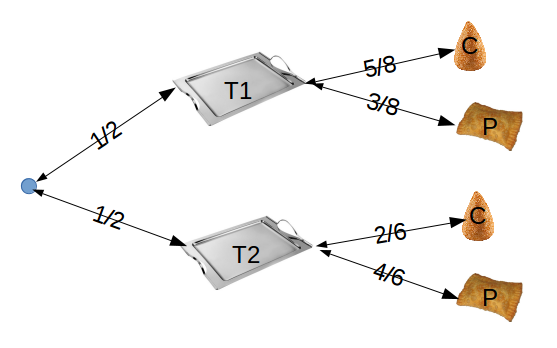
\includegraphics[width=0.6\paperwidth]{coxinha.png}
\end{figure}

Então:

$\displaystyle P(P)=P(P/T1)+P(P/T2)=(\frac{1}{2} \times \frac{3}{8})+(\frac{1}{2} \times \frac{4}{6})=\frac{25}{48}$

\section*{Exercício 12 - Quando $P(A)=1/2, P(B)=3/4$ e $P(A \cup B)=1$, quanto vale?}

\subsection*{a) $P(A \cap B)$}

$\displaystyle P(A \cup B)=P(A)P(B)-P(A \cap B)$

$\displaystyle P(A \cap B)=P(A)P(B)-P(A \cup B)$

$\displaystyle P(A \cap B)=\frac{1}{2} \times \frac{3}{4} - 1$

$\displaystyle P(A \cap B)=\frac{1}{4}$

\subsection*{b) $P(A^c \cap B^c)$}

Seja $P(A^c \cap B^c) = P[(A \cup B)^c]$

$\displaystyle  P[A \cup B] = 1 -  P[(A \cup B)^c]$

$\displaystyle  P[(A \cup B)^c] = 1 - P[A \cup B]$

$\displaystyle P[(A \cup B)^c] = 1 - 1 = 0$


\subsection*{c) $P(A \cap B^c)$}

Seja $P(A \cap B) = 1/4$

$P(A \cap B^c) = P(A)-P(A \cap B) = 1/2-1/4=1/4$

\subsection*{d) $P(A^c \cap B)$}

Seja $P(A \cap B) = 1/4$

$P(A^c \cap B) = P(B)-P(A \cap B) = 3/4-1/4=1/2$

\subsection*{e) $P(A | B)$ e $P(B | A)$}

Seja $P(A \cap B) = 1/4 = P(B \cap A)$

$\displaystyle P(A | B) = \frac{P(A \cap B)}{P(B)}=\frac{1/4}{3/4}=1/3$

e

$\displaystyle P(B | A) = \frac{P(B \cap A)}{P(A)}=\frac{1/4}{1/2}=1/2$








\bibliographystyle{plain}
\bibliography{bibliography.bib}

\end{document}
